\section{Introduction} \label{sec:introduction}



Our society and economy are increasingly dependent on Artificial Intelligence (AI). Correspondingly, AI models are becoming more accessible to the public at large while leveraging more complex architectures and consuming significant computational resources \cite{strubell-etal-2019-energy, strubell2020energy, yarally2023uncovering}. AI workloads raise significant sustainability concerns, thus exacerbating the already over-exploited resources of our planet \cite{buchholz_extreme_2024, schwartz2020green, dhar2020carbon}. Besides, AI workloads raise economic concerns with training and inference of massive-scale models in the scale of hundreds of millions of dollars in compute resources \cite{patterson2021carbon, schwartz2020green}. For example, the cost of training GPT 4.5 is estimated at \$500 million \cite{villalobos_how_2024}, Gemini 2.0 at \$200-300 million \cite{yogatama_economics_2025}, and DeepSeek R1 at \$50-80 million \cite{yogatama_economics_2025}.


\begin{figure}
    \centering
    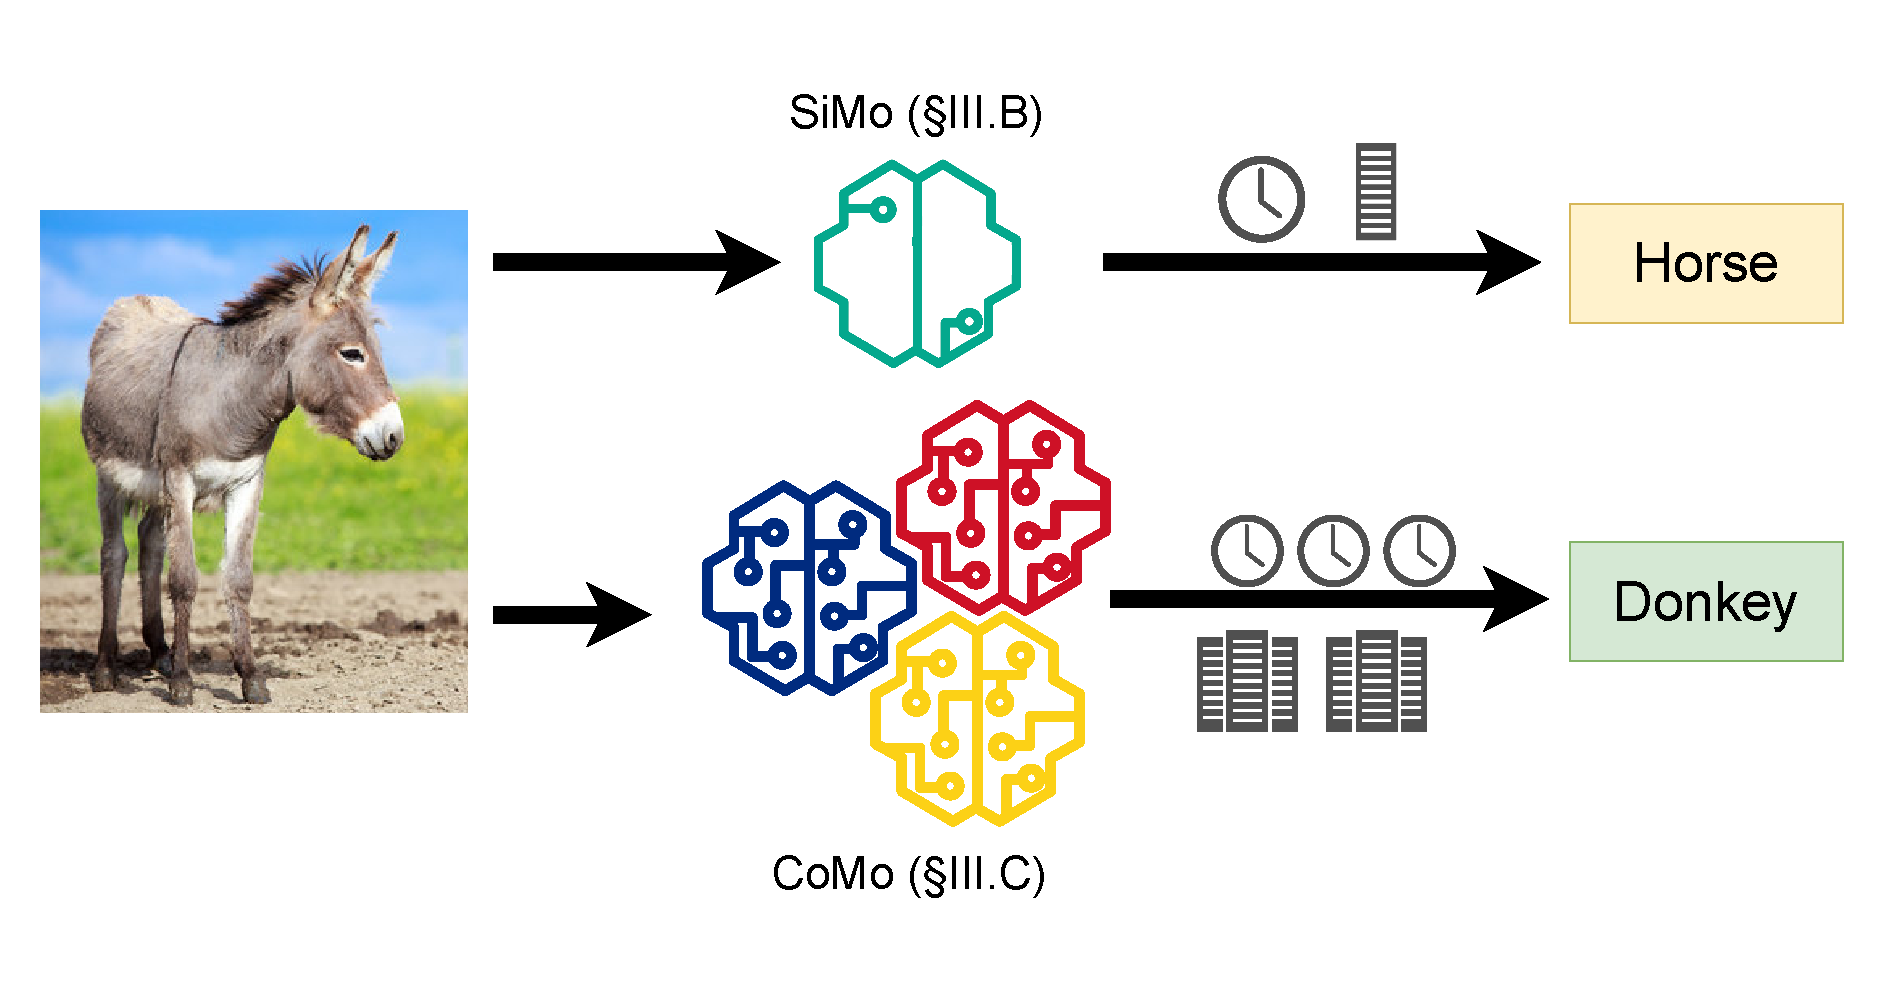
\includegraphics[width=0.98\linewidth]{figures/figure1-simo-como-hi-level.pdf}
    \vspace{-0.2cm}
    \caption{SiMo uses a simple architecture for prediction, while CoMo aggregates multiple complex models; architectural difference cascade into different accuracies and different computational resources.}
    \label{fig:high-level-element}
    \vspace{-0.6cm}
\end{figure}

\begin{figure*}
    \centering
    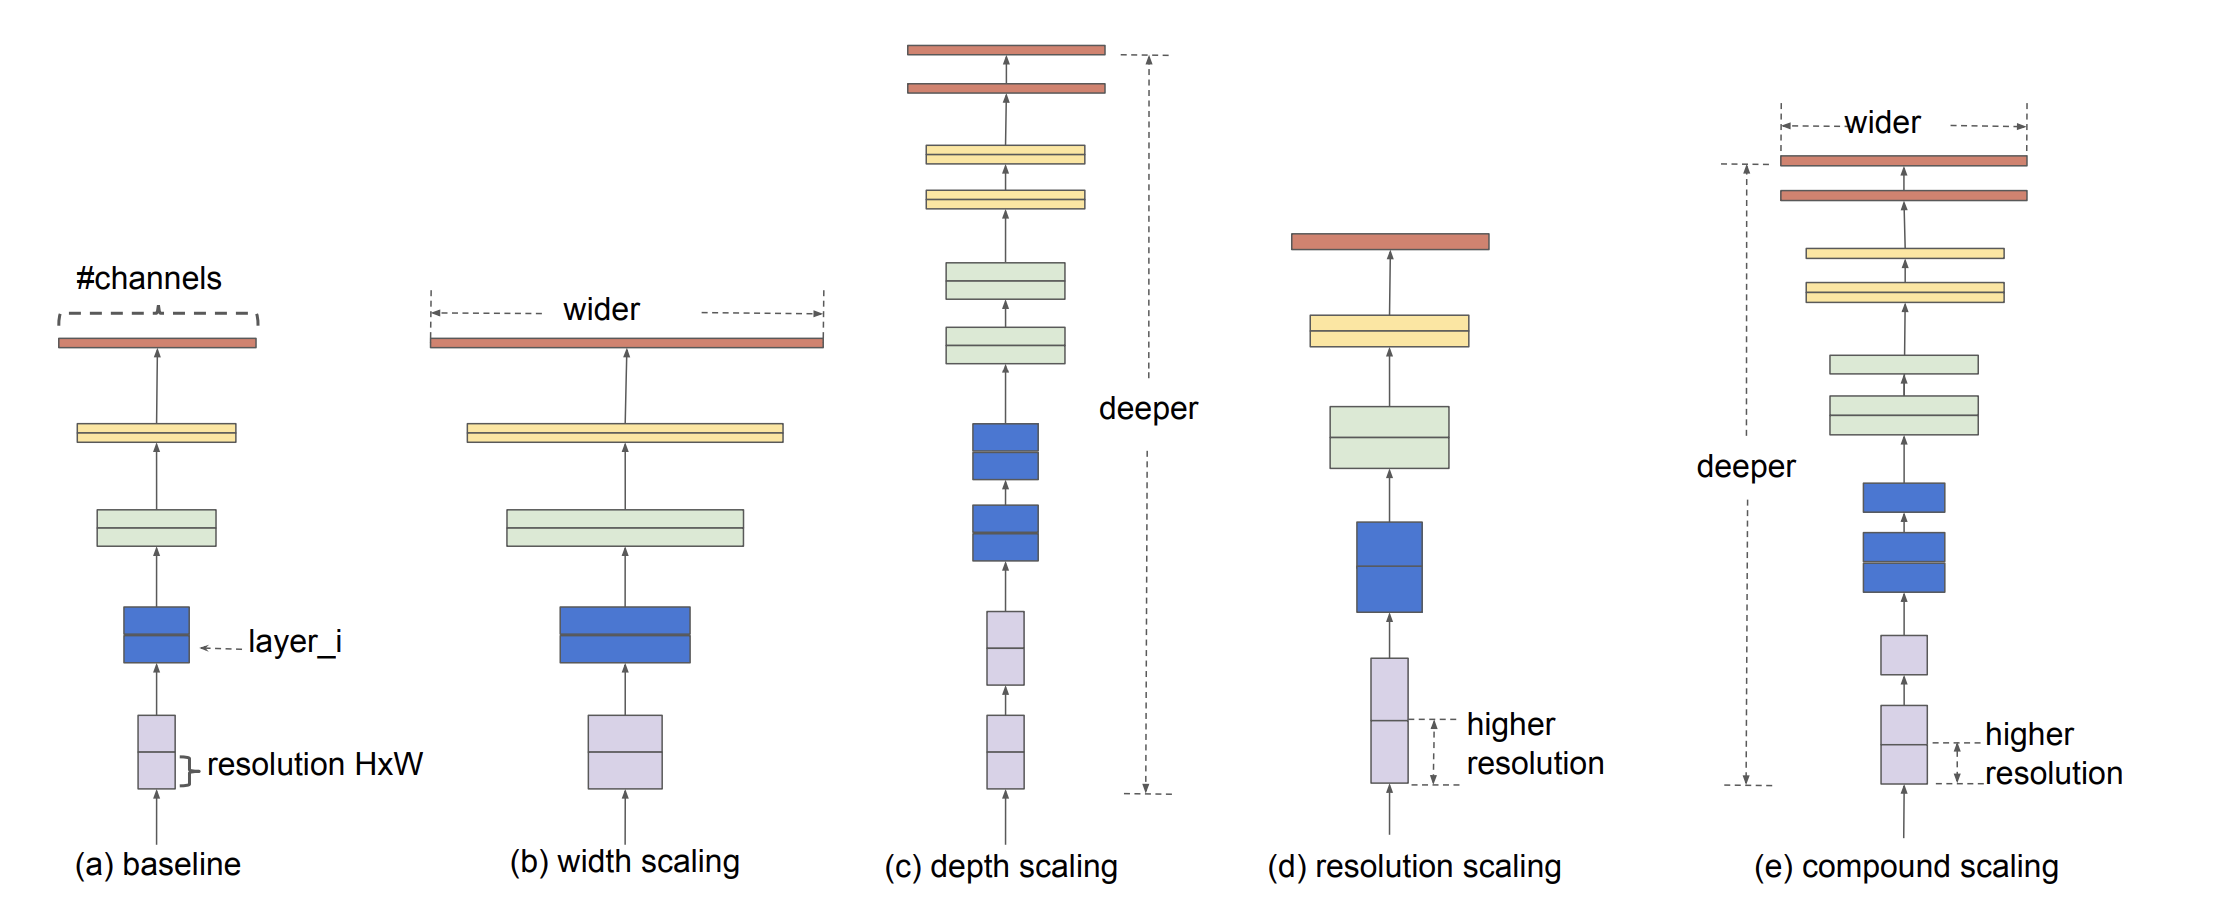
\includegraphics[width=0.95\linewidth]{figures/f2.png}
    \caption{EfficientNet architecture, for B0-B7, extracted from~\cite{luntz1969estimation}. In this work, we leverage and aggregate B0-B3 into CoMo.}
    \label{fig:background:f2}
\end{figure*}

To address the high environmental and financial cost, researchers and engineers analyze tradeoffs between employing simple architectural models, involving less computational expenses, yet having poor(er) accuracy, and employing complex architectural models, with better accuracy, yet with high computational expenses. These tradeoffs are encountered both in phases of training and inference, especially when the systems are scaled to millions of users. Object recognition is an increasingly common  application, with significant practical relevance in emerging and evolving fields of metaverse \cite{2024-hotcloudperf-metaverse-trace, 2023-hotcloudperf-metaverse}, augmented reality \cite{grigorescu2020survey, tomtom_augmented_2023}, or autonomous driving \cite{mao20233d}. In these fields, the current state-of-the-art involves adopting complex-architectural models, which offer higher accuracy at the cost of increased computational resources, energy consumption, and financial investment, without systematically exploring a middle ground in the complexity spectrum \cite{krishna2023complementary, schwenker20013d}. Addressing this gap, in this work, we design, prototype, and evaluate two contrasting architectural models for object recognition: SiMo and CoMo. 

Figure 1 illustrates our approach through an analogy. SiMo and CoMo receive an image for prediction (e.g., a donkey). SiMo, prioritizing performance over accuracy and unable to distinguish small nuances, predicts \textit{horse}, using minimal time and computational resources. CoMo, prioritizing accuracy over performance, predicts \textit{donkey} but uses more time and computational resources. 

\textit{Open challenge: The lack of tradeoff analysis, especially in the application domain of object recognition using AI / ML.} This raises the main research question (MRQ):

\begin{enumerate}[label=\textbf{MRQ}]
\item \label{introduction:mrq} How to explore the impact of architectural complexity on the accuracy and performance of deep learning models?
\end{enumerate}

To answer MRQ, we formulate three research questions (RQ) and centralize our research towards answering:

\begin{enumerate}[label=\textbf{RQ\arabic*}]
\item \label{introduction:rq1} How to design a simple- (SiMo) and a complex- (CoMo) architectural deep learning model for object classification?
\item \label{introduction:rq2} How to prototype SiMo and CoMo?
\item \label{introduction:rq3} How to evaluate and compare SiMo and CoMo?
\end{enumerate}

\textit{Approach and main contribution:} In this work, we address the open challenge by designing, implementing, and evaluating the tradeoff between SiMo and CoMo with a three-fold contribution:

\begin{enumerate}[label=\textbf{C\arabic*}]
\item \label{introduction:c1} (\textbf{Design}) We design SiMo and CoMo, two AI models with different architectural complexities for object classification (\Cref{sec:design}). We formulate functional and non-functional requirements and propose an overall architecture for SiMo and CoMo. SiMo employs a lightweight CNN architecture aimed for efficiency, while CoMo leverages an ensemble of 4 pretrained models to maximize accuracy.

\item \label{introduction:c2} (\textbf{Experimentation}) 
We obtain an open-source, peer-reviewed dataset for object classification, select methods for data augmentation, and split the result into train-validation-test sets (\Cref{sec:implementation:collection}, \ref{sec:implementation:augmentation}, \ref{sec:implementation:division}). We engineer a prototype of SiMo and CoMo, and train models (\Cref{sec:implementation:training}). The three experiments: (i) Evaluate the trade-off between training resources and model accuracy (\Cref{sec:experiments:exp1}); (ii) Analyze the tradeoff between inference time and prediction accuracy (\Cref{sec:experiments:exp2}); (iii) Compare the accuracy of individual models aggregated by CoMo with the composite, complex model itself (\Cref{sec:experiments:exp3}). 

\item \label{introduction:c3} (\textbf{Open Science}) 
We obtain an open-source, peer-reviewed dataset for object classification, select methods for the data used and created in this project. We release both SiMo and CoMo implementations together with training and evaluation scripts to ensure reproducible science. We also make available our training and evaluation scripts and provide a dataset tailored for object classification used in this work. Lastly, we make available the interactive results overview \footnote{\url{https://wandb.ai/fzovpec/ml_project}} that also includes the model weights samples every 20 training epochs, allowing for full experiment reproducibility following the principles of open science.


\end{enumerate}




